\chapter{Results and Analysis}
\label{ch:results}
\glsresetall
\section{Preamble}

The simulation and measurement results are captured using the methods described in sections 2 and 3. A comparison between the simulation and measurement targets is completed by calculating the correlation of each targets frequency vector, at each angle. This correlation function results in a single correlation coefficient for each angle.

Generally, the correlation coefficient is below one (a perfect match between measurements). Missile 1 showed the highest correlation between its measurement and simulation, with a mean correlation coefficient of 0.862, and standard deviation of 0.092. The mean correlation of the succeeding targets decreased with each continuously, with missile 5 showing the lowest mean correlation of 0.082, and standard deviation of 0.234.

These breakdowns in correlation between measurement and simulation are expected to impact the capability of the classifier. A classifier will be considered a `failure` if it cannot exceed an accuracy of $20\%$, equivalent to randomly guessing the targets label.

\section{Measurment Results}
\label{sec:meas_res}

	Figures \ref{fig:n1}, \ref{fig:n2}, \ref{fig:n3}, \ref{fig:n4}, and \ref{fig:n5} represent the calibrated RCS measurements of missiles 1, 2, 3, 4, and 5 respectively. Each figure include a plot of the vertically and horizontally polarized radar configuration.

	The measured values are converted to RCS for the purpose of display using \ref{eq:ieee_rcs}, with a transmitted signal of $E_t = 1 [V/m^2]$, and converted to $RCS [dB_{sm}]$ using

	\begin{equation}\label{eq:rcs_db}
		RCS [dB] = 10 * \log \left( \frac{RCS [m^2]}{1 [m^2]}\right)
	\end{equation}

	The green sector represent the RCS data that is used to train the machine learning model. The RCS polar plots show only one frequency. The total frequency content of each target over all angles are shown in figures \ref{fig:c1}, \ref{fig:c2}, \ref{fig:c3}, \ref{fig:c4}, and \ref{fig:c5}. Again, figures are shown in $RCS [\textrm{dB}_{sm}]$ represent the calibrated RCS measurements of missiles 1, 2, 3, 4, and 5 respectively. Each figure include a plot of the vertically and horizontally polarized radar configuration.

	The measurement result shows deteriorated performance for all measurements taken over the vertically polarized wave. This is a defect of the instrumentation radar:  the amplifier bank has been experiencing deteriorated performance due to a defect in the hardware. This was known prior, but the collection was taken anyway in an attempt to utilize the results to a limited extent, and to quantify the breakdown in performance.

\section{Simulation Results}
\label{sec:sim_res}

    Figures \ref{fig:ns1}, \ref{fig:ns2}, \ref{fig:ns3}, \ref{fig:ns4}, and \ref{fig:ns5} represent the simulated RCS of missiles 1, 2, 3, 4, and 5 respectively. Each figure include a plot of the vertically and horizontally polarized radar configuration.

		As with the measurement data, each plot is converted to $dB_{sm}$ using equation \ref{eq:rcs_db}.

\section{Data Comparison}
\label{sec:data_comparison}

	As described in section \ref{sec:comparison}, the correlation-per-angle of each target between its simulated and measured data is taken. The average correlation product per target ($<\rho>$) is plotted against SNR for each target, and shown in figure \ref{fig:correlation_results_snr}.

	\begin{figure}[htbp!]
    \centering
    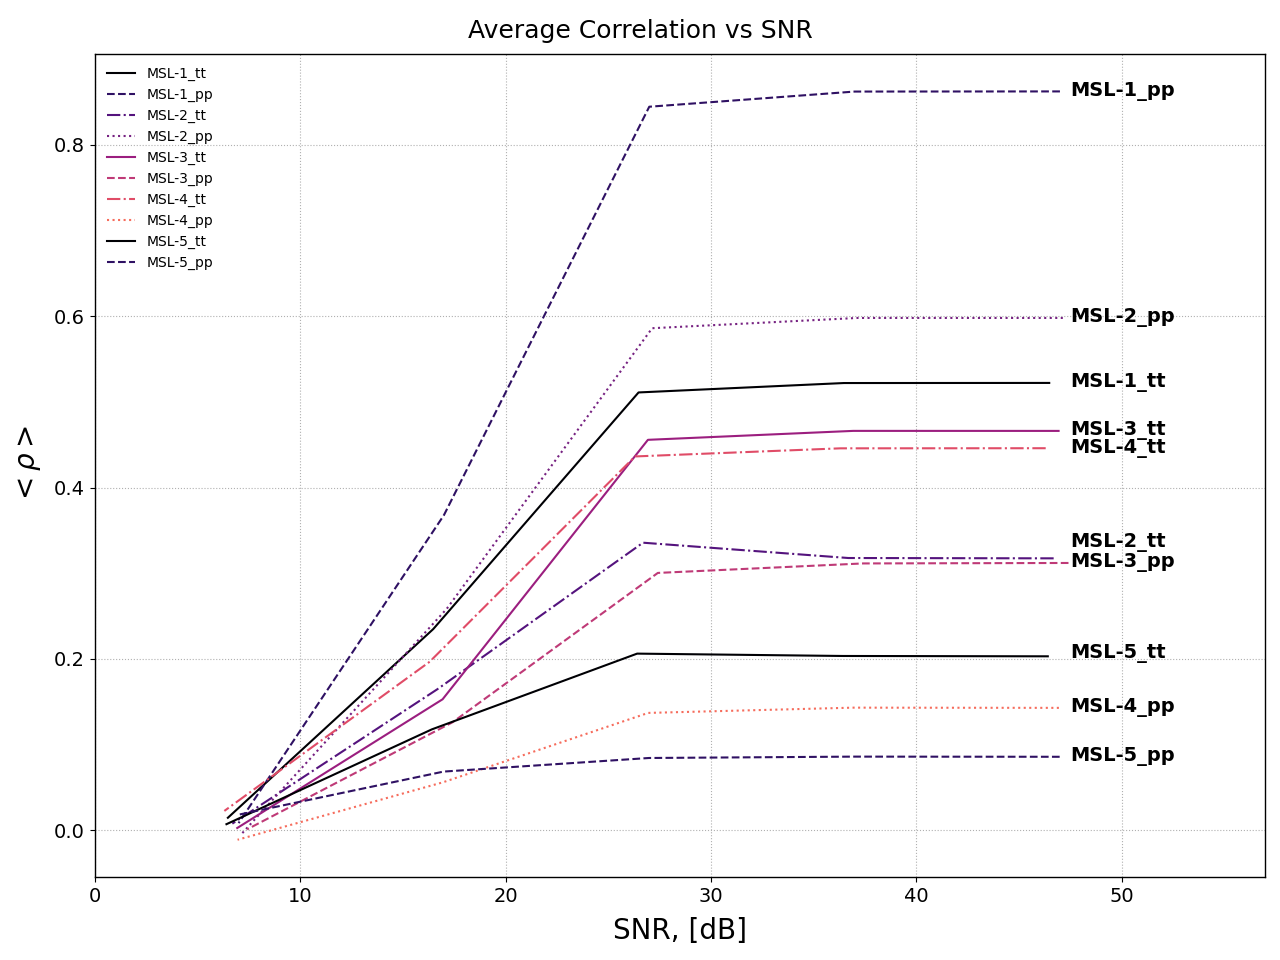
\includegraphics[width=.8\linewidth]{Correlation_vs_SNR.png}
    \caption[Average Correlation vs SNR]{Top-down and side view of the AFIT compact radar range.}
    \label{fig:correlation_results_snr}
  \end{figure}

	As expected, the average correlation between the simulated and measured data increases with SNR. At a roughly $28 dB$, correlation performance is flat. All targets show a near complete breakdown in correlation around $6 dB$. Surprisingly, the vertically polarized measurements have a higher average correlation than expected. There is however a decay in correlation performance as the target designator increases. Missile 1 'pp' shows the strongest correlation with an average $\rho$ of 0.892. This is followed by Missile 2 'pp' with an average $\rho$ of 0.6. The remaining measurements fall between an average $\rho$ of 0.6 and 0.08.

 	%TODO:  determine if I need to put the total graphs in the report, or draw on them later.
	%TODO:  be prepared to explain the breakdowns in correlation and how this will impact the classifier


\section{Model Evaluation}

	The hyperparameters of each model were determined using brute-force. The parameters for \textit{Sample Size}, \textit{Learning Rate}, \textit{Batch Size}, as well as the optimizer were evaluated using multiple values, and tested on data set.

	\subsection{VGG-19}

		The test parameters for the VGG-19 are shown in table \ref{tab:vgg-19_params}

		\begin{table}[htbp!]
			\begin{center}
				\caption[Hyperparameter test factors]{List of test factors used to evaluate model performance.}
				\label{tab:corrs}
				\begin{tabular}{|r|l|}
					\hline
					\textbf{Paramters} & \textbf{Value}\\
					\hline
					Sample size	&	1000 \\
											& 3000 \\
											& 5000 \\
					\hline
					Learning Rate	& 0.1 \\
												& 0.01 \\
												& 0.001 \\
					\hline
					Batch Size	&	100 \\
											& 200 \\
											& 300 \\
					\hline
					Optimizers	& `Adam` \\
											& `RMS Prop`\\
											& `SGD` \\
					\hline
					Momentum 	& 0.5 \\
										& 0.7 \\
										& 0.9 \\
					\hline
				\end{tabular}
			\end{center}
		\end{table}



		The parameters above were placed into a test matrix, and passed to the model. Only one parameter is changed per evaluation in order to identify trends in performance. Each evaluation is completed 5 times in-order to statistically characterize the model's performance for the given parameters.

		The training data for each evaluation has a progressively larger amount of AWGN applied. The purpose of the noise is to identify performance in the presence of hostile noise, and also to create random variance in the training data.

		The VGG-19 was only able to converge when using the SGD optimizer, which was then used for the remainder of testing. The values of momentum are applicable to the SGD optimizer only.

		Preliminary testing was conducted to reduce the number of test factors that would be evaluated. Learning rates below 0.001 showed poor convergence, and resulted in failed classifications.
